%!TEX root = report.tex
\subsection{Extrinsic Calibration}
\label{sec:extrinsic}
\subsubsection{Reference Points}

\paragraph{Points} 
In a first run, 4 to 6 bright orange circular reference points where used for the extrinsic calibration. The points are numbered and the first 2 points serve as the basis for the reference frame. (see Figure \ref{fig:ref_points}).

Since the distances between all points can be very accurately measured using a laser pointer, the euclidean distance matrix is set up and the absolute positions in the reference frame are obtained using the classical Multidimensional Scaling (MDS) method. \cite{Wickelmaier2003}

The limitations of this method are that the number of reference points can only hardly be extended since all points need to be numbered manually by the user and the number of laser pointer measurements increases quadratically.
Secondly, the radius of the reference points needs to be chosen big enough to be robustly detected from distance. But increasing the radius leads to a higher imprecision since the points can not be exactly placed on the ground and are perceived at different heights from different camera angles.

\paragraph{Checkerboard}
A more accurate and more user friendly approach using a checkerboard for reference points was therefore implemented. 
Since many robust implementations exist for checkerboard corner detection, its use promises a big number of reference points with minimal effort and high reliability. 
In addition to that, the checkerboard corners are of much smaller radius than circular reference points and can be placed exactly on the ground.

In order to avoid the manual numbering of all checkerboard points an automatic procedure based on three reference points placed in the corners of the checkerboard is implemented. 
The three reference points are detected manually and the numbering starts at the chessboard corner closest to point 1, goes on in direction of point 2 and then up in direction of point 3 (Figure \ref{fig:ref_checkerboard.png}).

\begin{figure}[htb]
	\centering
	\begin{subfigure}[b]{0.49\linewidth}
        \centering
		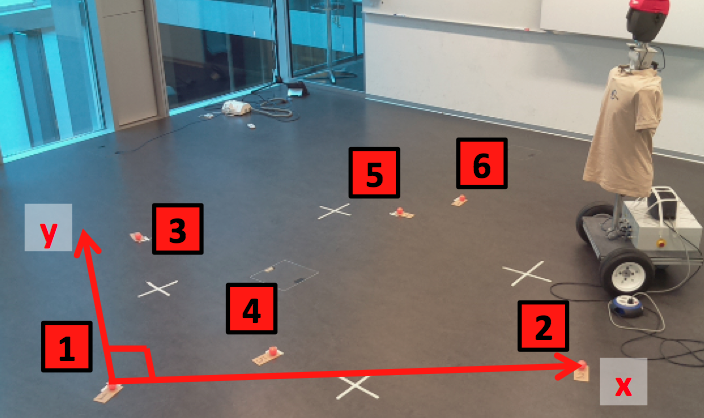
\includegraphics[height=0.6\linewidth]{files/ref_points.png}
		\caption{Reference points reference frame}
        \label{fig:ref_points}
	\end{subfigure}
	\begin{subfigure}[b]{0.49\linewidth}
        \centering
		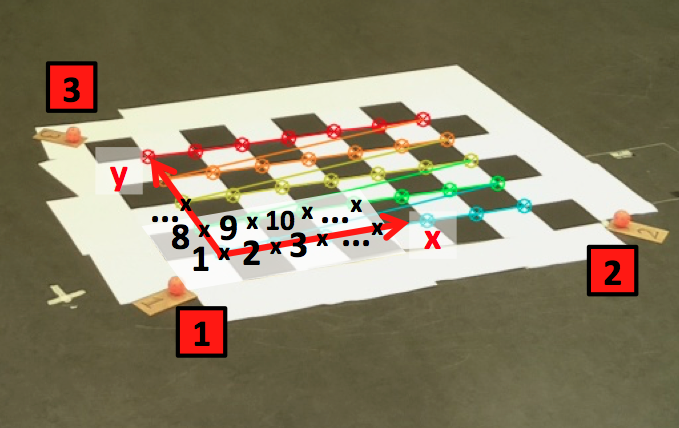
\includegraphics[height=0.6\linewidth]{files/ref_checkerboard.png}
		\caption{Checkerboard reference frame and numbering}
		\label{fig:ref_checkerboard.png}
	\end{subfigure}
	\caption{Reference point and checkerboard layout conventions.} 
\end{figure}

\subsubsection{Algorithm}

The reference points are detected as explained in § \ref{sec:imageprocessing}. The so found image-object space correspondances can be used to determine the camera position and orientation by solving the following system of equations for $R$ and $\mathbf{t}$.
\begin{align}
    \mathbf{x_i} = proj(\mathbf{X_i},P)& = C \quad P \quad \mathbf{X_i} \\
    s_i \begin{bmatrix} u_i \\ v_i \\ 1 \end{bmatrix} &= 
    C \begin{bmatrix} R \quad|\quad \mathbf{t} \end{bmatrix}
    \begin{bmatrix} X_i \\ Y_i \\  Z_i \\ 1 \end{bmatrix}, \quad \text{for }i=1\cdots N_{pts},
    \label{eq:projection}
\end{align}

where $N_{pts}$ is the number of points (4 to 6 or number of checkerboard corners), 
$\begin{bmatrix} u_i & v_i & 1 \end{bmatrix} ^T$ are the homogenous image coordinates with scaling factor $s_i$ and $\begin{bmatrix} X_i & Y_i &  Z_i & 1 \end{bmatrix} ^T$ are the homogenous object point cooridnates. $C$ is the intrinsic camera matrix, determined as explained in \ref{sec:intrinsic}.

The extrinsic camera matrix $P$ that one needs to solve for can be decomposed in a rotation and a translation component.
\begin{align}
    R &= \begin{bmatrix} 
        r_{11} & r_{12} & r_{13} \\
        r_{21} & r_{22} & r_{23} \\
        r_{31} & r_{32} & r_{33} \\
    \end{bmatrix} \quad \text{Camera rotation matrix}\\
    \mathbf{t} &= \begin{bmatrix} 
        t_1 & t_2 & t_3
    \end{bmatrix} ^T \quad \text{Camera translation vector}
    \label{eq:solvepnp}
\end{align}

The camera center in object space coordinates is then given by

\begin{equation}
    \begin{bmatrix} x_C & y_C & z_C \end{bmatrix}^T = -R^{-1} \mathbf{t}.
\end{equation}

There are 12 unknowns and each new point provides 3 independant equations. Therefore at least 4 points are requried for solving this problem.

Various methods have been proposed for solving this Perspective-$n$-Point or P$n$P problems. 
The methods can be embedded in a Ransac scheme, which makes them more resistant to outliers. 
However, outliers will not occur in the present experimental setup because of its deterministic nature: all reference points are precisely defined and need to be detected, as opposed to setups where a undefined amount of feature points are extracted from images.

Three different methods for solving this P$n$P problem are implemented in \texttt{OpenCV}.
\texttt{P3P} is based on a technique that is limited to 4 points only, so it was immediately rejected. The \texttt{EPNP} method \cite{Lepetit2009} provides a non-iterative solution to the problem which is more stable and computationally inexpensive. Since in the present case, the number of points is limited to 40 and the calculation time turned out to be acceptable, the method chosen is the \texttt{ITERATIVE} method, based on reprojection error minimization.

The reprojection error is the sum of the squared distances between observed projections $\mathbf{x_i}=[u_i,v_i,1]^T$ and the projected object points ($\mathbf{proj}(\mathbf{X_i},P)$), defined as in \eqref{eq:projection} and calculated with the current estimation of the extrinsic camera matrix $P$. Formally, this means

\begin{equation}
S(\boldsymbol\beta) = \sum_{i=1}^{N_{pts}} \| \mathbf{x_i}-proj(\mathbf{X_i},P(\boldsymbol\beta)) \| ^2 ,
\end{equation}

and the optimization problem can be written as
\begin{equation}
    \hat{\boldsymbol\beta} = \underset{\beta} {\mathrm{argmin}} ~S(\boldsymbol\beta).
\end{equation}

For an adequate convergence in all directions, this minimization problem is solved with the Levenberg-Marquardt algorithm, also called damped least-squares. The optimization parameters are the entries of the matrix $P$, which are grouped in the vector $\boldsymbol\beta$. At each minimization step a \"damped\" update of the parameter vector $\boldsymbol\beta=\boldsymbol\beta_{old}+\boldsymbol\delta=$ is used depending on the decent of the optimization function, as defined in \eqref{eq:LMA} \cite{LMA}
\begin{equation}
    (J^TJ + \lambda \mathbf{diag}(J^TJ))\boldsymbol\delta = J^T[\mathbf{x}-\mathbf{proj}(\mathbf{X},P)]
\label{eq:LMA}
\end{equation}

where $J$ is the Jacobian matrix of the reprojection function and $\lambda$ is the damping factor. It is tuned such that
the convergence is moderated in the case of very fast descending functions, preventing from instability, and enhanced for slowly converging problems.
